\documentclass[a4paper]{article}
\usepackage[margin=3cm]{geometry}
\usepackage{xcolor}
\usepackage{graphicx}
\usepackage{lipsum}
\usepackage{amsmath}
\usepackage{pdfpages}
\usepackage{url}
\usepackage{hyperref}
\usepackage{subcaption}
\usepackage[font=small,labelfont=bf]{caption}
\usepackage{siunitx}
\hypersetup{
    colorlinks = true,
    colorlinks = false,
	linkbordercolor = {white},
	urlcolor = {blue},
	linkcolor = {blue},
	citecolor = {blue}
}
\usepackage{acronym}
\usepackage[acronym,nomain]{glossaries}
\makeglossaries
\newcommand{\todo}[1]{\textbf{\textcolor{red}{#1}}}
%\newcommand{\td}[1]{\textbf{\textcolor{red}{#1}}}
\newcommand{\td}[1]{\textcolor{red}{#1}}
\newcommand{\me}[1]{\textcolor{gray}{#1}}
\newcommand{\ds}[1]{}
\newcommand{\x}{$\times$}
\newcommand{\picwidth}{0.7\textwidth}

%SI UNITS
\newcommand{\cm}[1]{\SI{#1}{\centi\meter}}
\newcommand{\mm}[1]{\SI{#1}{\milli\meter}}
\newcommand{\mg}[1]{\SI{#1}{\milli\gram}}
\newcommand{\ml}[1]{\SI{#1}{\milli\liter}}
\newcommand{\um}[1]{\SI{#1}{\micro\meter}}
\newcommand{\ul}[1]{\SI{#1}{\micro\liter}}
\newcommand{\minutes}[1]{\SI{#1}{\minute}}
\newcommand{\oc}[1]{\SI{#1}{\degreeCelsius}}
\newcommand{\s}[1]{\SI{#1}{\second}}
\newcommand{\h}[1]{\SI{#1}{\hour}}

\title{Functional oxide layers for electrical isolation and chemical passivation of steel substrates}
\author{Johann Dorn}

\begin{document}
\maketitle
\newacronym{zrpro}{Zr(PrO)$_4$}{zirconium(IV)propoxide}
\newacronym{acac}{Hacac}{acetylacetone}
\newacronym{acoh}{AcOH}{acetic acid}
\newacronym{buoh}{BuOH}{1-buthanol}
\newacronym{ipo}{IPO}{2-Propanol}
\newacronym{ito}{ITO}{indium doped tin oxide}
\newacronym{fto}{FTO}{fluorine doped tin oxide}
\newacronym{n2}{N$_2$}{nitrogen}
\newacronym{water}{H$_2$O}{deionized water}
\newacronym{sds}{SDS}{sodium dodecyl sulfate}
\newacronym{hcl}{HCl}{hydrochloric acid}
\newacronym{h2so4}{H$_2$SO$_4$}{sulfuric acid}
\newacronym{naoh}{NaOH}{sodium hydroxide}
\newacronym{zro}{ZrO$_2$}{zirconium dioxide}
\newacronym{1f}{1F}{one-fold concentrated solution}
\newacronym{2f}{2F}{two-fold concentrated solution}
\newacronym{3f}{3F}{three-fold concentrated solution}
\newacronym{4f}{4F}{four-fold concentrated solution}
\newacronym{5f}{5F}{five-fold concentrated solution}
\newacronym{db}{DB}{doctor blading}
\newacronym{pv}{PV}{photovoltaic}
\newacronym{cigs}{CIGS}{copper indium gallium sulfide}

\newacronym{sg}{SG}{sol-gel}
\newacronym{ftir}{IR}{Fourier transform infrafred}
\newacronym{sem}{SEM}{scanning electron microscopy}
\newacronym{xrd}{XRD}{X-ray diffraction}

\newacronym{pso}{PSO}{particle swam optimization}
\newacronym{ml}{ML}{machine learning}



\clearpage
\section*{Abstract}
%\lipsum[1]
\td{A thin zirconium oxide layer was applied via doctor blading on a steel foil substrate with the goal of get an moeglichst homogeneous and insulating layer.
The layers were characterized over the current-voltage curve and the operational variables were optimized with an pso swarm optimization algorithm.
}
\section*{Preface}
\lipsum[2]
%Thank
%I want to thank Theodoros Dimopulos, Adhi, Neha, Philipp. 
%Quyhn, Maria, Jana, Vivien and Katharina who tried to keep me sane throughout the
%Elif 
%This project showed how import is to plan experiments, chose fitting methods, reproducablitiy and how import proper reseaerch and constant reading of literature is. 
\clearpage
\tableofcontents
\clearpage
\printglossaries
\clearpage
%%%%%%%%%
%%%%%%%%%%%%%%%%%%%%%%%%%%%
%%%%%%%%%%%%%%%%%%%%%%%%%%%%%%%%%%%%%%%%%%%%%%%%%%%%%%

%%%%%%%%%
%%%%%%%%%%%%%%%%%%%%%%%%%%%
%%%%%%%%%%%%%%%%%%%%%%%%%%%%%%%%%%%%%%%%%%%%%%%%%%%%%%
\section{Introduction}
\td{describe everything what is mentioned in \ref{sec:exp}}
\Gls{pv} is one big hope when trying to become carbon neutral as it uses the energy provided by sun directly in contrast to renewable energy sources (e.g. wind and water) or even carbon based sources.
One sort of \gls{pv} are \gls{cigs} \cite{Vasekar2010} cells. % https://doi.org/10.1016/j.tsf.2009.09.033}
In order to make a module, multiple cells are operated in series. 
The cells must be applied to a non-conducting surface.
Glass is a good non-conducting substrate, but very rigid and brittle. 
An alternative is steel, which is ductile, inexpensive and highly available, but conducting. 
An insulating layer must therefore be applied to the steel substrate before any \gls{cigs} cells can be applied.
A non-toxic material which is suitable for this application is \gls{zro}. 
An economic and scalable method is doctor blading via a \gls{sg} process. 
\gls{sg} processes often produce porous layers. 
In this work a dense, insulating and homogeneous layer is pursued. 
ML can help to uncover complex non-linear relations, such as the influence of the production factors on the thickness and resistance of the resulting layer.
The minisation of the conductance if performed with a particle swarm optimization algorithm.
%%%%%%%%%
%%%%%%%%%%%%%%%%%%%%%%%%%%%
%%%%%%%%%%%%%%%%%%%%%%%%%%%%%%%%%%%%%%%%%%%%%%%%%%%%%%
\section{Aims and Objectives}
The aim of this work is to develop a non-conducting layer on steel based on  non-toxic materials like Aluminium or Zirconium via doctor blading. 
This layer can then be used as insulator for CIGS modules on steel sheets.
Doctor blading - or tape casting - is a widely used precision coating method to apply thin films on large area surfaces\cite{Berni2004}.
%The method of doctor blading, which is in principle a sol-gel process, 
This sol-gel process was chosen because of the availability to the industrial partner.
In order to optimize the resulting layer the multitude of parameters was optimized with an particle swarm optimization ansatz. %machine learning 
The conductivity (dependent variable), the number of layers and calcination time (both independent variables) should be minimized.
%The conductivity should be as small as possible.
%The number of layers should be held small and the calcination heating rate should be maximized. 
\iffalse
Defensio: Argumente in der Arbeit noch mal sichten, Feedback von Betreuungsperson im Kopf haben - da könnten Fragen kommen, 
sich selbst aufnehmen 

Präsentieren: Visualisierungen sinnvoll? 
Antworten überlegen/Argumente überlegen
Limitation, Rahmen der Arbeit
Begründung für die eigene Vorgehensweise
\fi
%%%%%%%%%
%%%%%%%%%%%%%%%%%%%%%%%%%%%
%%%%%%%%%%%%%%%%%%%%%%%%%%%%%%%%%%%%%%%%%%%%%%%%%%%%%% EXPERIMENTAL
\section{Theoretical Background aka How does is work?}
%\url{https://link.springer.com/content/pdf/10.1186/2228-5326-3-8.pdf}
\subsection{Sputtering}
\subsection{SEM}
\url{https://doi.org/10.1016/B978-0-12-816806-6.00017-0}\\
\subsection{Infrared absorption}
\subsection{X-Ray Diffraction}
\url{https://doi.org/10.1016/B978-0-12-816806-6.00017-0}\\
\url{https://chem.libretexts.org/Courses/Franklin_and_Marshall_College/Introduction_to_Materials_Characterization__CHM_412_Collaborative_Text/Diffraction_Techniques/X-ray_diffraction_(XRD)_basics_and_application}\\
\subsection{Particle Swarm Optimization}
\subsection{Machine Learning}
\subsection{Princlipal Component Analysis}

%%%%%%%%%%%%%%%%%%%%%%%%%%%
%%%%%%%%%%%%%%%%%%%%%%%%%%%%%%%%%%%%%%%%%%%%%%%%%%%%%%
\clearpage
\section{Experimental}
\label{sec:exp}
In this section the used chemicals and substrates, experimental procedures and any used equipment are described. 
\subsection{Substrate Preparation}
Five different substrates were used throughout this work: 
microscope glass slides (\cm{2.5}\x\cm{7.5})\ds{ from Sigma Aldrich},\ds{ thinner,} squared glass plates (\cm{2.5}\x\cm{2.5})\ds{ from Sigma Aldrich}, \gls{ito} glass plates (\cm{2.5}\x\cm{2.5})\ds{ from Sigma Aldrich}, \gls{fto} glass plates (\cm{5}\x\cm{5})\ds{ from Sigma Aldrich} and steel foil (10~cm~x~10~cm) provided by Sunplugged GmbH (\url{http://sunplugged.at/)}.
The glass slides and \gls{fto} were scored with a diamond scribe \ds{\td{(diamond scratcher/scraper)} }and broken with a running plier into pieces of dimensions \cm{2.5}\x\cm{2.5}.
The steel foil was cut with a foil cutter.
%, a cutter knife (repeatedly), a paper cutter or a scissors (ordered by increasing curvature of resulting plates).
All substrates were cleaned in three steps before usage:
\begin{enumerate}
	\item \minutes{15} in \ml{50} \gls{water} and \ml{1} of Hellmanex III alkaline concentrate in a sonic bath
	\item \minutes{15} in \gls{water} in a sonic bath
	\item \minutes{15} in \gls{ipo} in a sonic bath 
\end{enumerate}
After the last cleaning step, the samples were blown dry with dry \gls{n2} gas and kept in a clean plastic container until the doctor blading step.

%%%%%%%%%%%%%%%%%%%%%%%%%%%
%%%%%%%%%%%%%%%%%%%%%%%%%%%%%%%%%%%%%%%%%%%%%%%%%%%%%%
\subsection{Solutions}
%Two main recipes were used and their compositions were varied. 
All recipes for solutions can be divided into two categories:
the first recipe - adopted from Anwar et. al. \cite{Anwar2017} - was based on \gls{zrpro} in \gls{acac} and \gls{water}.
The second recipe - adopted from Hu et. al. \cite{Hu2016} - was based on \gls{zrpro} in \gls{buoh}.

\begin{figure}[htb]
	\centering
	\begin{subfigure}{0.49\textwidth}
		\centering
		%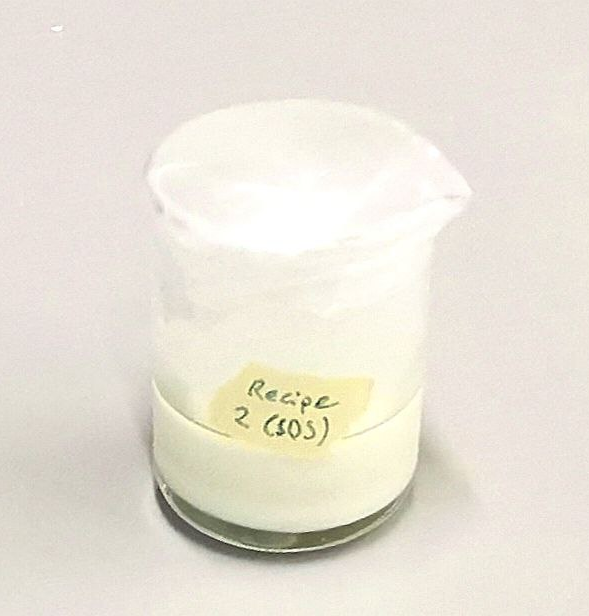
\includegraphics[width=.99\textwidth]{Pics/sol-aq.png}
		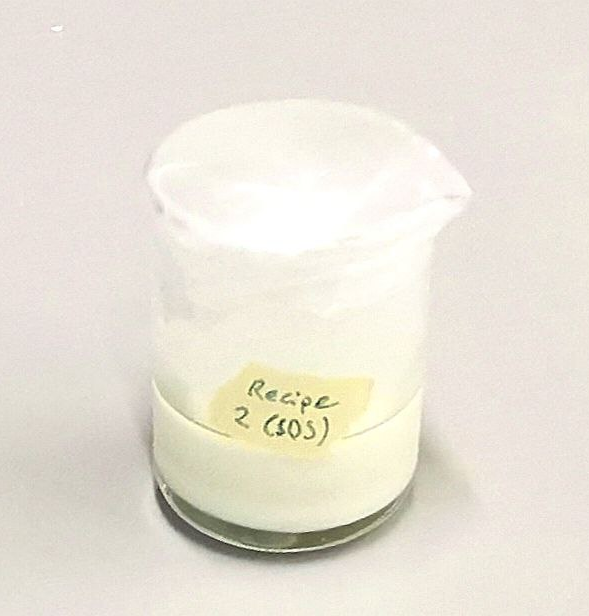
\includegraphics[height=0.8\textwidth]{Pics/sol-aq.png}
		\label{fig:sol-aq}
		\caption{Aquatic solution}
	\end{subfigure}
	\begin{subfigure}{0.49\textwidth}
		\centering
		%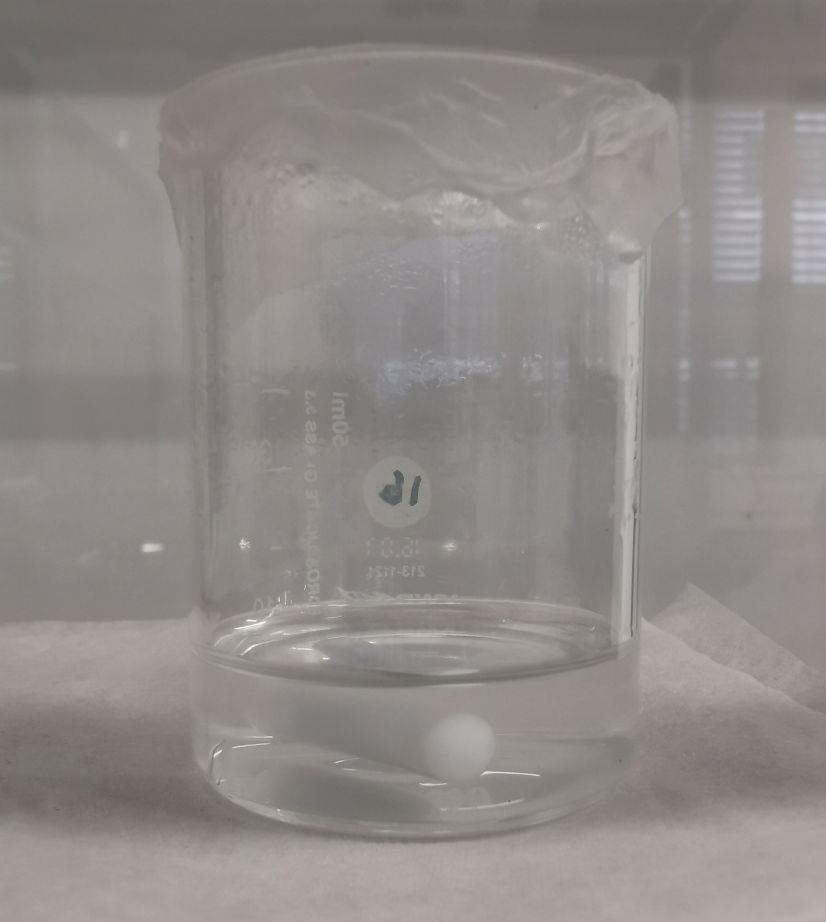
\includegraphics[width=.99\textwidth]{Pics/sol-bu.png}
		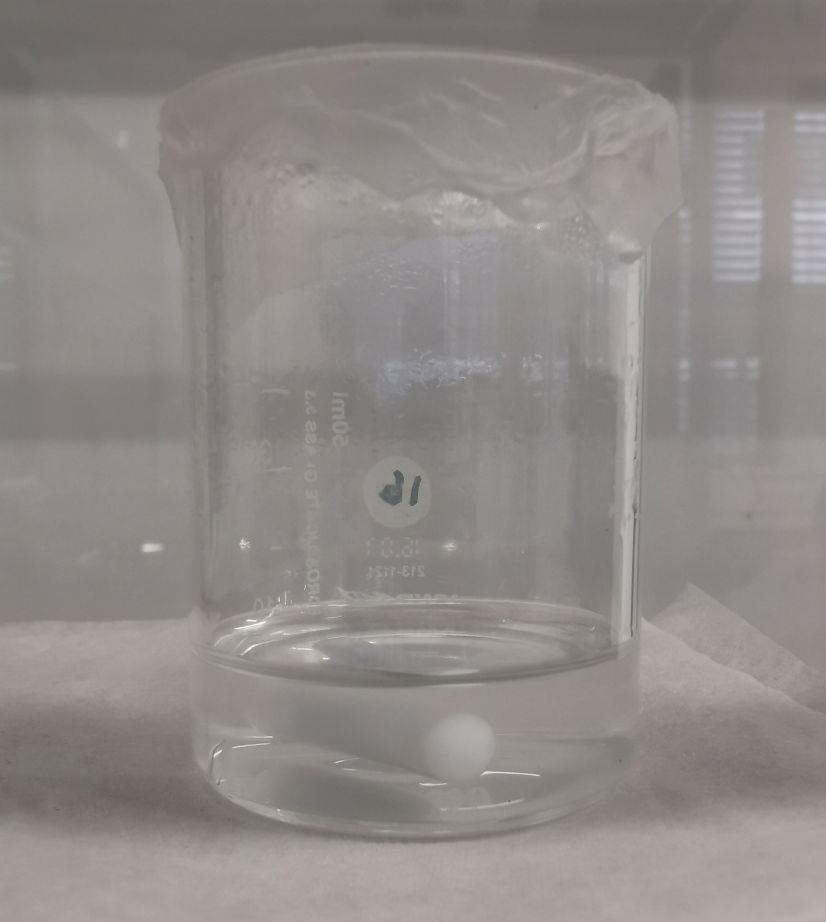
\includegraphics[height=0.8\textwidth]{Pics/sol-bu.png}
		\label{fig:sol-bu}
		\caption{Buthanolic solution}
	\end{subfigure}
	\label{fig:sol}
	\caption{Aquatic and buthanolic solution in beaker glass with magnetic stirring bars sealed with Parafilm} 
\end{figure}

%%%%%%%%%%%%%%%%%%%%%%%%%%%%%%%%%%%%%%%%%%%%%%%%%%%%%%
\subsubsection{Aquatic solution}
%\me{The procedure for the aquatic solution is as follows:}
\gls{zrpro} was added to \gls{acac} while stirring and in a separate vessel \gls{water} (including any optional additives such as \gls{sds}, \gls{hcl}, \gls{h2so4} or \gls{naoh}) was added to \gls{ipo} and both were stirred for one hour. 
The \gls{water}-\gls{ipo} mixture was added to the other solution and stirred over night. 
The exact volumes can be taken from table~\ref{tab:rec1}.
\td{At this point in time everything was doctor bladed by hand. The hight was varied (with tape).
Chemicals were added to influence pH and surface tension with the goal to influence the resulting layer. }
\begin{table}[h]
	\centering
	\caption{Compositions of different aquatic solutions}
	\label{tab:rec1}
	\begin{tabular}{llllllll}
		\hline
		recipe				&1		&2		&3		&4		&5		&6		&7\\
%		\hline
%		conc. [a.u.]	&1		&1.7	&2.6	&3.5	&4.4	\\
		\hline
		\gls{zrpro} [\ml{}]	&8		&8		&8		&8		&8		&8		&8\\
		\gls{acac}  [\ml{}]	&8		&8		&8		&8		&8		&8		&8\\
		\gls{ipo}   [\ml{}]	&2		&2		&2		&2		&2		&2		&2\\
		\gls{water} [\ml{}]	&2.6	&2.6	&2.5	&2~		&2		&2		&2\\
		\gls{sds}   [\mg{}]	&-		&5.9	&-		&-		&-		&-		&-\\
		\gls{hcl}   [\ml{}]	&-		&-		&-		&-		&0.5	&-		&-\\
		\gls{h2so4} [\ml{}]	&-		&-		&-		&-		&-		&0.5	&-\\
		\gls{naoh}  [\ml{}] &-		&-		&-		&-		&-		&-		&0.5\\
		\hline
	\end{tabular}
\end{table}
%
%%%%%%%%%%%%%%%%%%%%%%%%%%%%%%%%%%%%%%%%%%%%%%%%%%%%%%
\subsubsection{Buthanolic solution}
\label{sec:sol}
Five different concentrations of the buthanolic solutions were prepared. 
%The first solution \td{(standard concentration/ one fold/ 1F)} 
%followed the recipe loosely, which is described by Hu et al. \cite{Hu2016}.
%In order to obtain thicker \gls{zro} layers the \gls{zrpro} concentration in the starting solution was raised.
The \gls{1f} 
was closest to the recipe proposed by Hu et. al. \cite{Hu2016}. 
\td{p34
The second recipe was adopted to the chemicals available in the lap and potential less toxic.
The first thing was to get a recipe with similar ingredients, which were available. 
p34 why did i try \#8 vs \#9 
The solvent (1,2-BuOH,BuOH, PrOH) and the chalating agent (AcAc and citric acid) were varied 
Later in the process, the stabilisation compound was also varied (AcOH, iPOH)
}
The other four solutions (\gls{2f}, \gls{3f}, \gls{4f}, \gls{5f}) were similar with higher concentrations of \gls{zrpro} (see table \ref{tab:rec2}).
%%%%%%%%%%%%%%%%%%%%%%%%%%%%%%%%%%%%%%%%

\begin{table}[h]
	\centering
	\caption{}
	\label{tab:rec2}
	\begin{tabular}{rlllll}
		\hline
		recipe	&1F		&2F		&3F		&4F		&5F		\\
		\hline
%		conc. [a.u.]	&1		&1.7	&2.6	&3.5	&4.4	\\
%		\hline
		\gls{buoh} [\ml{}]		&4.95	&4.9	&4.85	&4.8	&4.75	\\
		\gls{zrpro} [\ml{}]	&0.05	&0.1	&0.15	&0.2	&0.25	\\
		\gls{acac} [\ml{}]		&0.0125	&0.025	&0.0375	&0.05	&0.0625	\\
		\gls{ipo}/\gls{acoh} [\ml{}]		&2		&2		&2		&2		&2		\\
		\hline
	\end{tabular}
\end{table}

%%%%%%%%%%%%%%%%%%%%%%%%%%%%%%%%%%%%%%%%
The solvent (\gls{buoh}) was put into a beaker glass (or similar, preferably with an 
air-tight cap) with a magnetic stirring bar and \gls{zrpro} was added while stirring. After 
stirring \minutes{\ds{10 to }15} one mole equivalent chelating agent (\gls{acac}) was 
added and stirred for another \minutes{\ds{10 to }15}. Finally, the stabilisation 
solvent\cite{Hu2016} (\gls{ipo} or \gls{acoh}) was added to the mixture and stirred for 
additional \minutes{\ds{20-}30}. 
%%%%%%%%%%%%%%%%%%%%%%%%%%%%%%%%%%%%%%%%
In order to make a \gls{2f} solution, the volume of \gls{zrpro} and \gls{acac} was 
doubled and \gls{buoh} was decreased by the volume of \gls{zrpro}. 

\subsection{Doctor blading}
\label{sec:DB}
An Erichsen Coatmaster 510 with a heatable plate was used for doctor blading. The plate 
had equally spaced circular \SI{2.5}{\milli\meter} diameter patches of porous metal where 
underpressure could be applied to keep substrate in place (see 
figure~\ref{fig:eric}). After setting the heating plate temperature, the vacuum plate 
temperature and the \gls{db} velocity, the \gls{db} blade 
was put into position, the sample was placed on the vacuum plate and the vacuum was 
switched on. %and the blade was sent over the sample without liquid to see if it was held in position. 
\ul{100} of solution were 
applied with a 10-\ul{1000} pipette and the blade moved over the sample distributing the 
liquid evenly. After evaporation of the solution, the vacuum was turned off, the 'blade 
pusher' put into initial position, the blade removed and excess solution removed with a 
wipe. The small metal plate was transferred to the hot heating plate and rested on there 
for 3-\minutes{5}. %The process can be repeated as wished. 
This process of applying a \gls{zro} layer was repeated as many times as needed.
\begin{figure}
	\centering
	\begin{subfigure}{.49\textwidth}
		\centering
		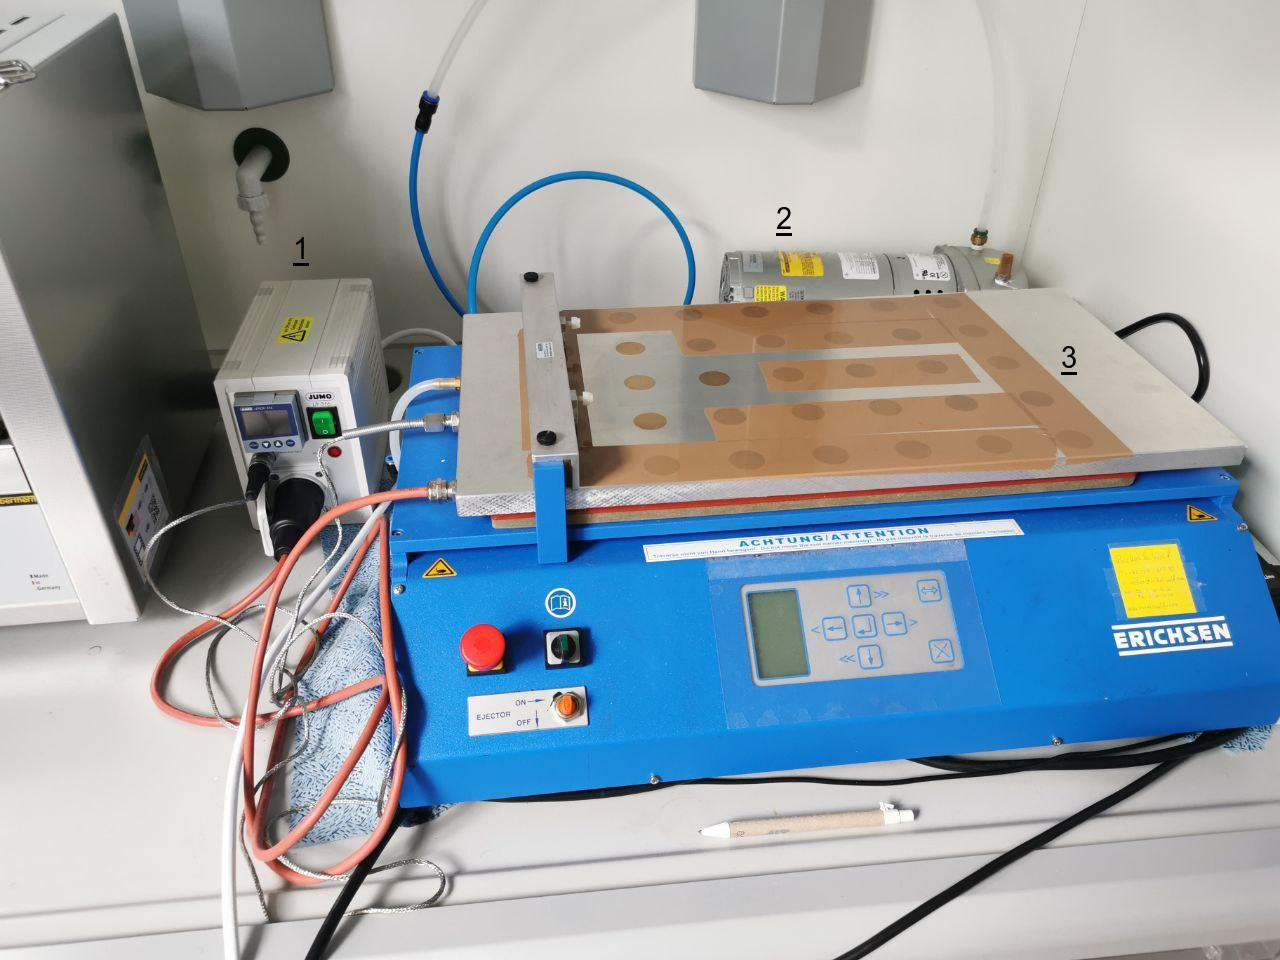
\includegraphics[width=.99\textwidth]{Pics/erichsen1.png}
		\caption{}
	\end{subfigure}
	\begin{subfigure}{.49\textwidth}
		\centering
		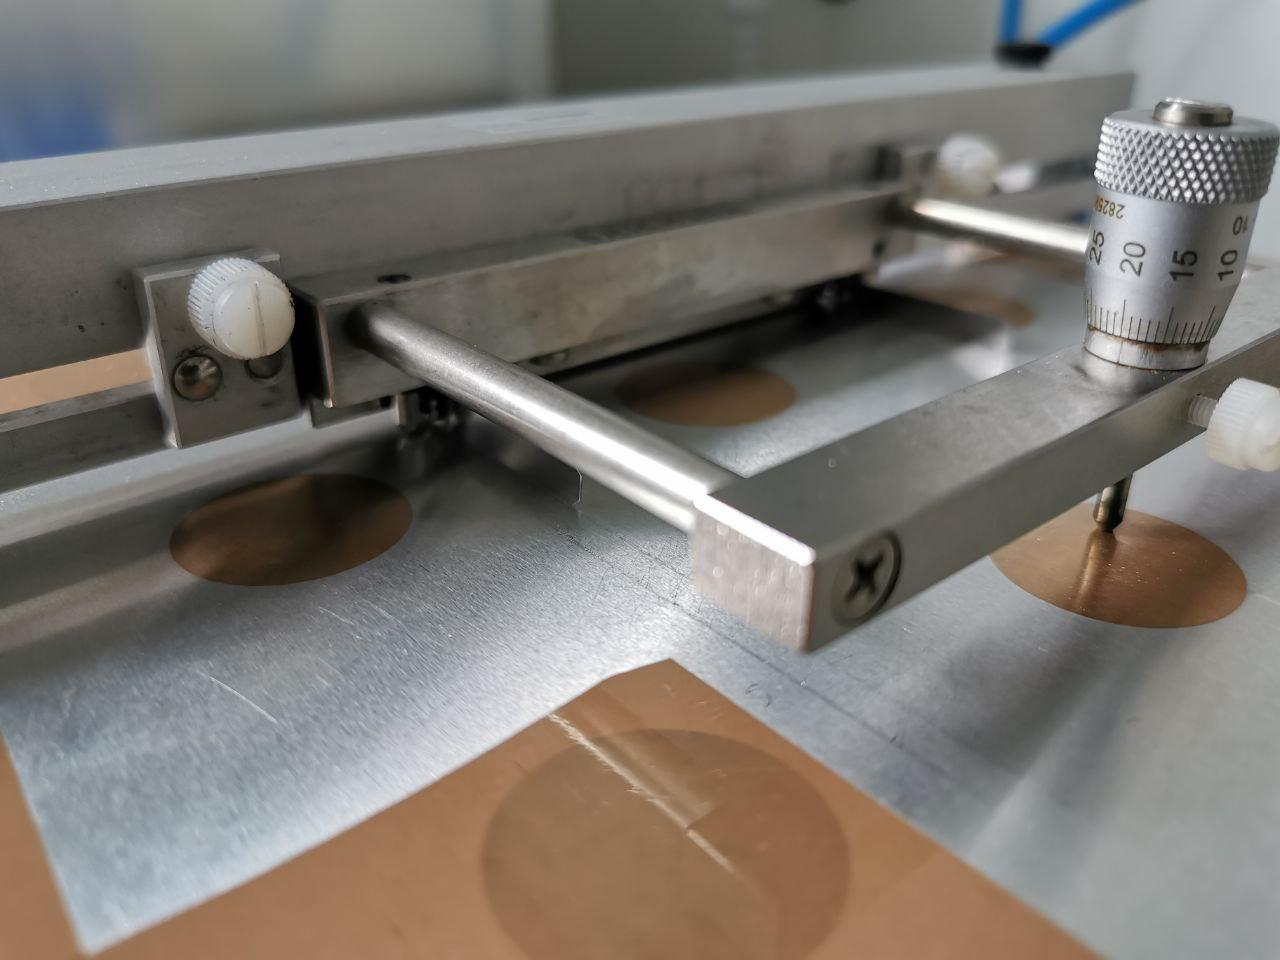
\includegraphics[width=.99\textwidth]{Pics/erichsendb1.png}
		\caption{}
	\end{subfigure}
	\caption{
		(a)
		Temperature regulator (1) on the left,
		vacuum pump (2) in the background and 
		Erichsen Coatmaster 510 (3) with heatable vacuum plate.
%		(b) Erichsen Coatmaster 510 with \gls{db} blade.
		(b) Close up of the \gls{db} blade in position.
		The majority of the suction areas is sealed with tape to increase the underpressure at the remaining ones.
	}
	\label{fig:eric}
\end{figure}

\subsection{Calcination}
A LabTech EH45C heating plate and a Naberterm LB410 furnace were used to calcinate the doctor bladed samples. 
%The heating plate heated with a steady rate of \td{\oc{5}/\minutes{}}.
%The heating plate can hold temperature for a certain amount of time, but doesn't have conifgurable heating rates.
The heating plate can hold temperature for a certain amount of time, but heated with a fixed rate of circa \oc{10}/\minutes{}.
In order to achieve a lower overall heating rate several temperature ramps and plateaus were alternated (see table~\ref{tab:labtech} and figure~\ref{fig:heat}).
%This procedure will be called HP1 from now on, which stands for heating plate procedure.
This procedure was called HP1.
The HP1 procedure was optimized for the available hardware by a colleague working on the project prior to the author.

\begin{table}[h]
	\centering
	\begin{tabular}{rl ll ll ll ll ll ll }%ll ll ll ll ll ll ll}
%			&temp [\oc]	&time/rate &temp [\oc]	&time/rate	&temp [\oc]\\
		HP1		&&&&&&&&&&&&&\\
		\hline
		T [\oc{}]	    &80		&100	&150	&160	&170 	&180	&190	&200	&250	&300	&350	&400	\\
		t [\minutes{}]	&10 	&10		&5 		&5 		&5 		&5 &5 &10 &10 &10 &10 &60 \\
		\hline
	\end{tabular}
	\caption{Time the temperature was held constant at certain temperatures on the heating plate}
	\label{tab:labtech}
\end{table}
%
The NT1 heating program was used to mimic the HP1 heating procedure in the Naberterm furnace. 
NT2 is an simplification of NT1 and programs NT3-NT6 are the same as NT2 with altered heating rate and partly increased calcination temperature T$_{\textrm{Cal}}$ (NT5).
NT2-NT6 had only 2 variables (heating rate and calcination temperature) instead of 4 (three different heating rates and calcination temperature). 
%where the \td{calcination time} was held constant.
%The time at maximum temperature was held constant over all heating procedures.
All heating programs were held at the calcination temperature for one hour.
In figure \ref{fig:heat} the different heating curves are depicted. 
%
%
\begin{table}[h]
	\centering
	\begin{tabular}{rl ll ll}% ll ll ll ll }%ll ll ll ll ll ll ll}
%			&temp [\oc]	&time/rate &temp [\oc]	&time/rate	&temp [\oc]\\
%		HP1		&&&&&\\%&&&&&&&&\\
%		\hline
%		T [\oc{}]				&80		&150	&200	&400	&400 	\\
%		$\theta$ [\oc{}/\minutes{}]	&10 	&10		&5 		&5		& 		\\
		\hline\hline
		Name	&80-150\oc{} [\oc{}/\minutes{}]	&150-200\oc{} [\oc{}/\minutes{}]	&200\oc{}-T$_{\textrm{Cal}}$ [\oc{}/\minutes{}]	&T$_{\textrm{Cal}}$ [\oc{}] &t$_{\textrm{Cal}}$ [\minutes{}]	\\
		\hline
		NT1		&2					&1					&2				&400	&60  \\
		NT2		&2					&2					&2				&400	&60  \\
		NT3		&3					&3					&3				&400	&60  \\
		NT4		&4					&4					&4				&400	&60  \\
		NT5		&4					&4					&4				&500	&60  \\
		NT6		&1					&1					&1				&400	&60  \\
%		NT7		&max				&max				&max			&600	&60  \\
		\hline\hline
	\end{tabular}
	\caption{Heating rates and calcination temperature holding times.}
	\label{tab:nt}
\end{table}

\begin{figure}
	\centering
	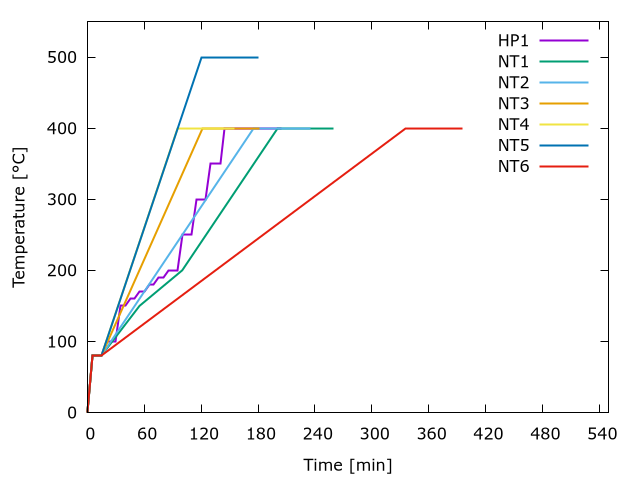
\includegraphics[width=.7\textwidth]{../Data/Graphs/hp1.png}
	\caption{Different heatings curves}
	\label{fig:heat}
\end{figure}

\subsection{Characterisation}
All \gls{sem} micrographs were taken with a Zeiss Supra 40. 
\Gls{ftir} transmitance and reflectance spectra were recorded with a Bruker Vertex 70 
%transmission [\%] and reflection?  which angle? 
spectrometer with a quartz beam splitter, \SI{0.5}{\milli\meter} aperture and 
Gallium-Phosphide detector for ultra violet light (\SI{303}{\nano\meter} - \SI{588}{\nano\meter})
and a Silicon detector for visual for 
% gallium phosphide http://dx.doi.org/10.1051/epjconf/20134800028
infrared light (\SI{500}{\nano\meter} - \SI{1.2}{\micro\meter}). For transmittance the light
entered the sample from the side with the layer. The UV and VIS+IR sepctra were merged via 
Opus software included in the spectrometer. 
%\td{IR around page 45
%REFLECTIVITY? can also be used for determination of thickness p47
%}
\Gls{xrd} spectra were obtained with a Thermo Scientific ARL Equinox 100 X-Ray Diffractometer. 
%The sample was placed in a way such that it absorbed half of the beam. 
All \gls{xrd} spectra were taken at \SI{5}{\degree} incident angle and compared to the internal database.
The current-voltage (I-V) curves were measured with Agilent 4156C Precision Semiconductor 
Parameter Analyzer. Prior to I-V measurements the samples were sputtered with aluminium 
through a mask to produce contact with a Leybold 
UNIVEX450C Sputter System.
Directional current sputtering with Argon as inert gas at \SI{0.005}{\milli\bar} with a 
power of \SI{40}{\watt} for \SI{700}{\second} was used. Between sputtering and I-V measurements 
direct contacts to the steel subtrate were created by removing the \gls{zro} layer on two 
opposing edge of a sample with sand paper and then by applying silver paste.
%\td{scratched until short circuit was produced (aka the steel foil was reached under the \gls{zro} layer).  }
\begin{figure}
	\centering
	\begin{subfigure}{0.48\textwidth}
		\centering
		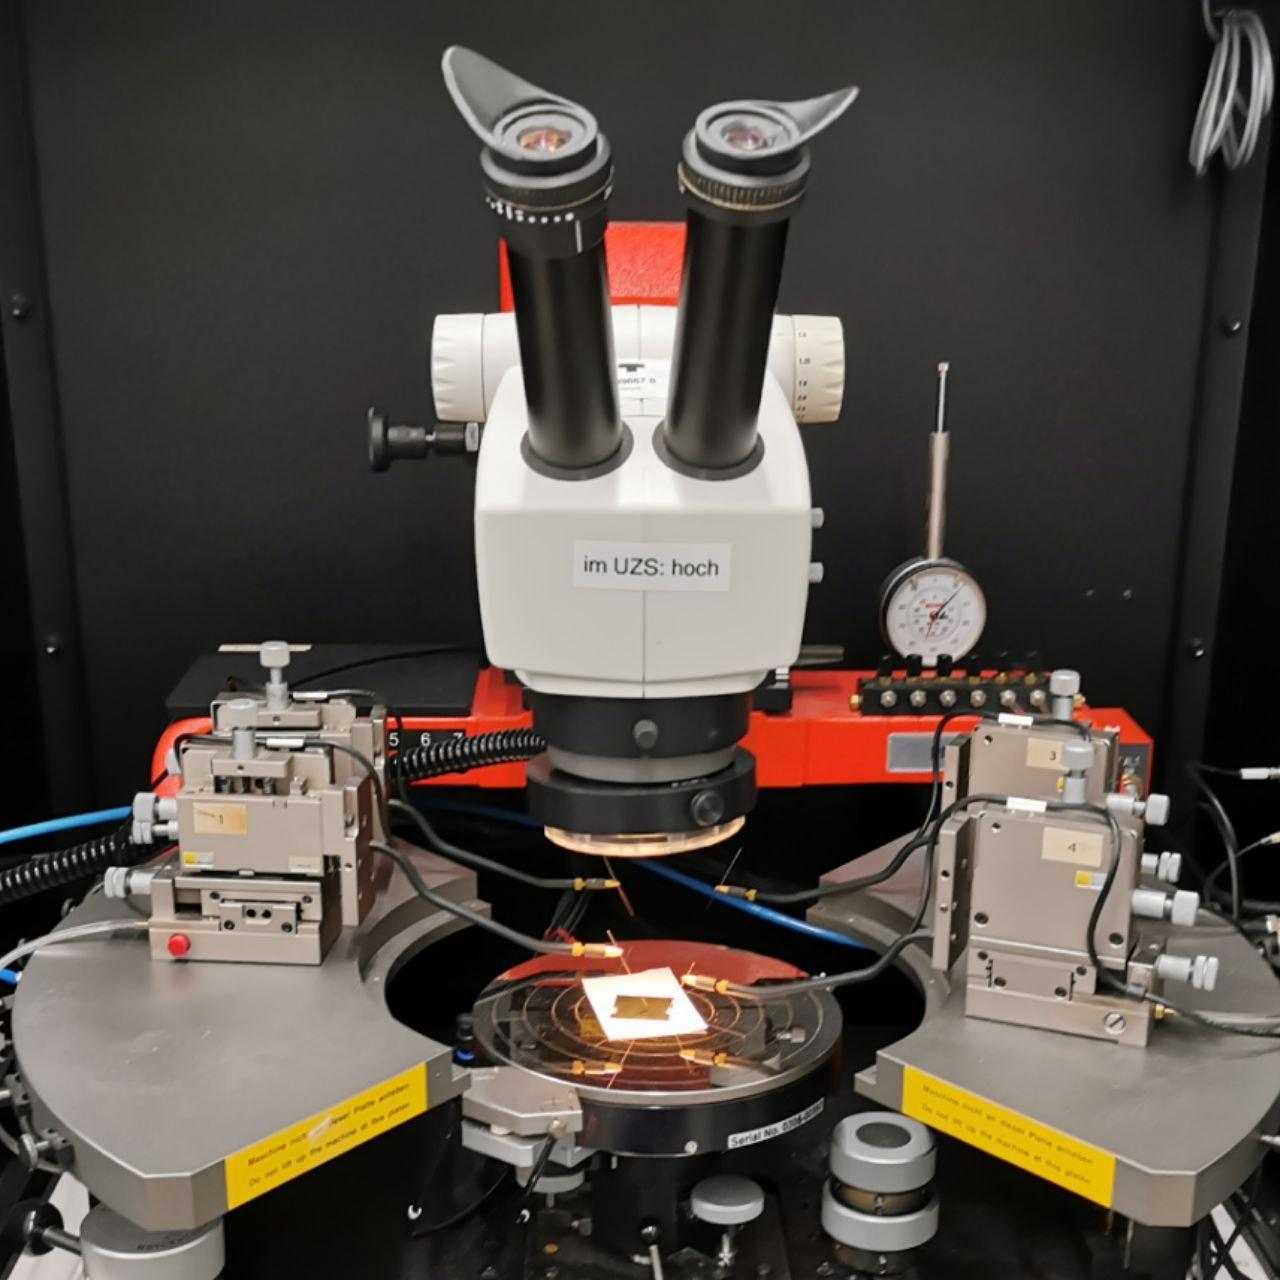
\includegraphics[width=.9\textwidth]{Pics/i-v.png}
		\label{fig:iv-agilent}
		\caption{peripherals}
	\end{subfigure}
	\begin{subfigure}{0.48\textwidth}
		\centering
		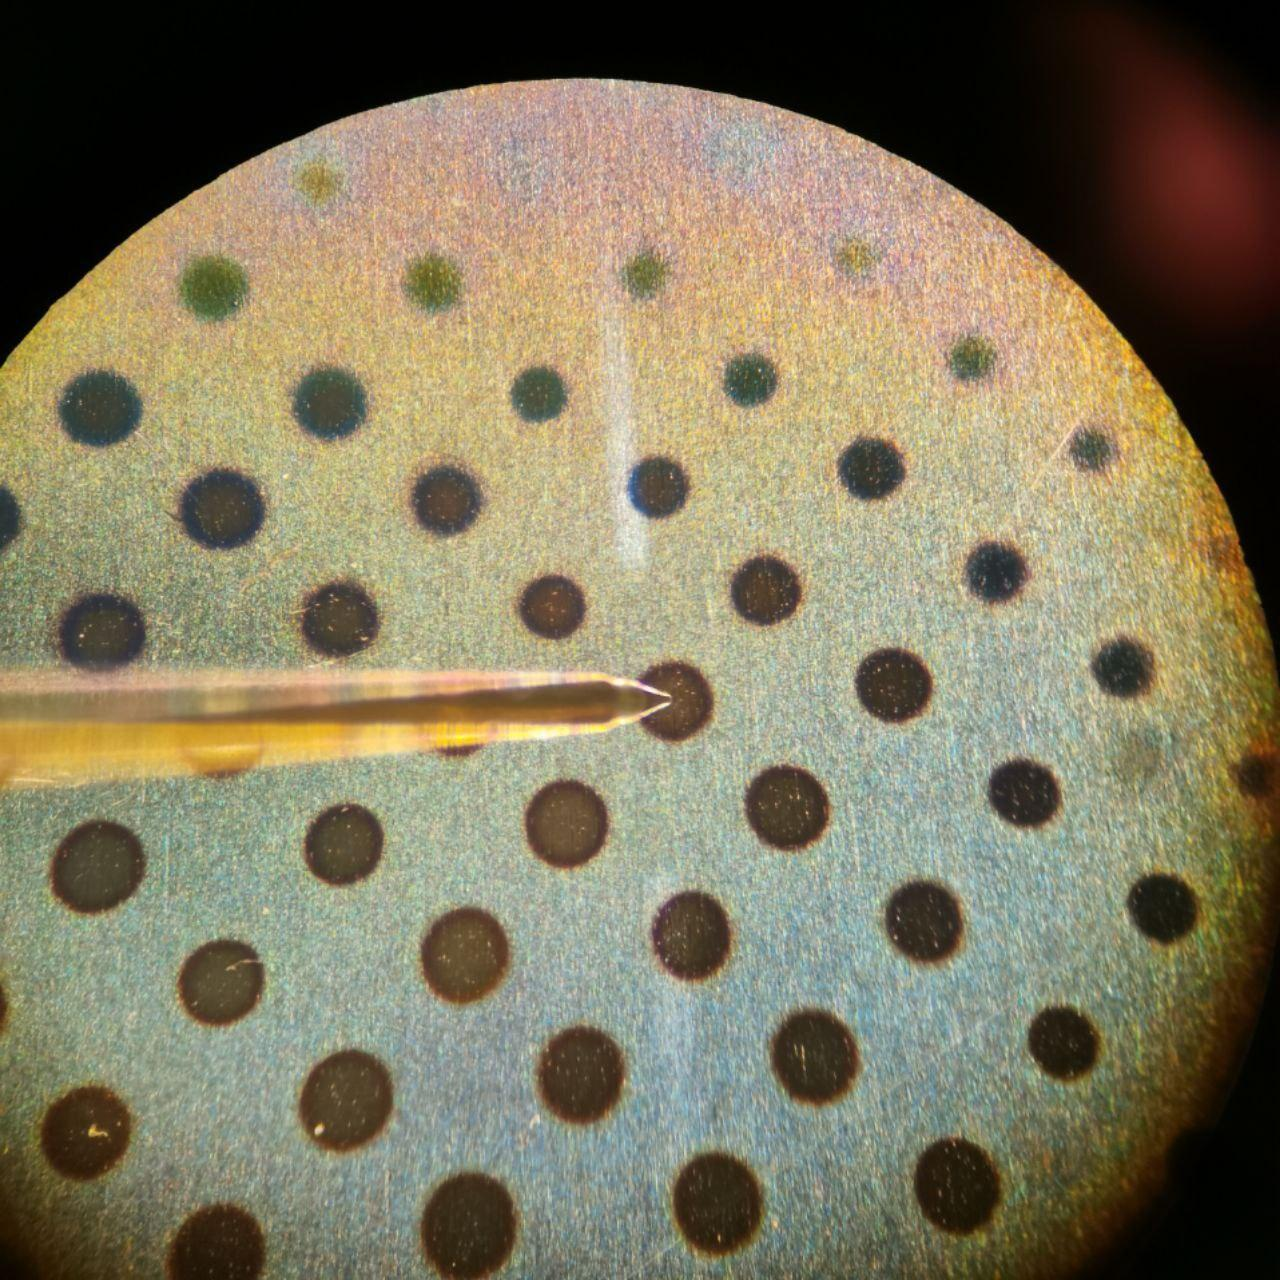
\includegraphics[width=.9\textwidth]{Pics/i-v-micro.png}
		\label{fig:iv-micro}
		\caption{View through the microscope}
	\end{subfigure}
	\label{fig:iv}
    \caption{I-V curve abnehm aperature and sicht durch das micro scope.\td{make a sketch}}

\end{figure}

%%%%%%%%%%%%%%%%%%%%%%%%%%%%%%%%%%%%%%%%%%%%%%%%%%%%%%%%%%%%%5
\subsection{Finding base process/Preliminary study}
Initially, glass plates were doctor bladed manually with aquatic solution and calcinated via HP1. 
Glass was used because of its availability and in order to be able to make IR \td{transmission} spectra.
In order to measure the resistivity of the produced layer \gls{fto} and \gls{ito} layered 
glass plates (both conductive) were used as substrate.
Conducting substrates were also needed to \gls{sem} produce micrographs. 
%otherwise the sample would charge and can't be pictured anymore. 
%this means if the produced layer is thick and homogeneous enough, it's difficult to see in sem
Different additives were included in the recipe (see table \ref{tab:rec1}) and the resistance was checked with a multimeter. 
\td{As no homogeneous layers resulted from any aquatic recipe} a new recipe was introduced, which gave more homogeneous films.
With this new buthanolic recipe the limits of the optimization problem were explored in a preliminary study.
%For the preliminary study a DB machine and NT were used and the steel. 
In the preliminary study only steel was used as substrate.
The Plackett-Burman design implemented in the python library \texttt{pyDOE} was used to
get an overview of reasonable boundaries.
%Latin squares were used to chose which experiments should be ausgefuehrt to get an ueberblick of the optimization room.
%See Code/Input_DOE/make_*exps.py and Code/Input_DOE/mail_theo
Some additional hand picked experiments were introduced to further narrow the limits of the optimization down as every reduction in variables or levels meant a faster convergence.
%ooooh 
\td{
acceptable layer was produced by solution, but very unstable (short lived) how long? p41 
extra AcOH stabilzed but needed so much that dilution to large...
The stirring time was untersucht, but not much difference so shortest was used because 
short time can produces faster and the resulting solution is longer stable 
(after finishing mixing)
10 layers were tried of short stiring and gave good results? samples 130,131,134,135 (p43)
}

\td{p48 started with erichson? 
used double sided tape to hold in place, which ofcourse gave extra thickness.
0-3.5 micro meter in 0.5 steps DB height were tested and did not substantially 
alter the results p 56
double calcination (2x400C) was tried instead of pyrolization (4x200 than 400C),p49
sooo higher concentration of zro2 leads to less stable solution
5F ca 100min
4F ca 140min
3F ca 7h 
}

\td{I-V: 2 terminal measurement 
one terminal was varibale and the other the ground 
from $-5*10^{-3}$ V to $5*10^{-3}$ V with steps of $10^{-2}$
measure current from back bone to backbone 
if shorted, then can measure actual resistance of layer. resistance of steel 
is neglectable. In order to get an impression of the quality of the layer 
mutliple contact (picture) are sputtered (throuhg a mask) and statistics: 
Two angabewerte: the weighted durchschnit and the number of pinholes, ie the number of contacts which were shorted, have an resistance below an threshold.
if tunneling, iv follows powerlaw, if direct contact, iv follows linear
}

\td{tryed to use heat gun to let solution evaporate faster, started to heat the DOC p55}
\td{varied doctor blading velocity: 10, 5, 1, 0.5, 0.2, 0.1. Slower less layer}

After a fitting recipe was found, the process to produce an acceptable layer was untersucht. 
There were many variables which had to be taken into account. 
The damals current procedure produced clear and continuous films, but was plagued from 
unhomogenities due to drying stains. 
Using a heat gunn the drying stain can be surcumvented (umgangen), but the results were unreproduceable. 
The glass unterlage was therefore exchanged with a metal plate which allowed both to hold the sample via underpressure and heat it to a certain temperature.
The bounds fore the process were then explored. 
Especially the doctor blading velocity.

\td{plachett-burman design of experiment with conc, layers, calcination temperature, 
heating rate, DB velocity and DB temperature as input variables.}
\td{base/best sample was somewhot 150, 5 layers 3F 2K/min 400C}
\td{p68 iPrOH to milky solution and solution becomes clear!!!! checked how much 
is needed. 5F solution milky over night ~2ml, added 1ml IPO and clear.}
\td{extra PB-design with conc(2-4), layers(6-8), tcal(430-470), tvel(4-6),
vdoc(0.5-2), tdoc(40-60). low vdoc very homogenuous but actually nearly no 
deposition because miniscus is pulling liquid off the substrate.}
\td{IPO influence on "stability" p74: 600ul IPO makes clear, 4000 ul BuOH not clear with 
same base solution (1ml of 4F), added extra 400ul to BuOH sol and after 5min clear. 
of 1:5 is unacceptable Dilution }
21.8 (1F) from 15.02. 13:30 bis 
26.3 (1ml iPO to ca2ml of 5f) from 16.02. 16:30 bis 18.02.++
18.02 4F in 80min milky
      2F in ca 24h (stabilization AcOH)
\td{In example of documentation 2 input variables and 1-2 responses initial population=10
, subsequent population=5, but 10 iterations. Clearly more input varibles and less 
iterations (as in actual experiments) lead to suboptimal results.
When plotting input vars  against the response variables, no trend
The exploration-vs-exploitation parameters of the model were also not set accordingly.}
see \href{https://search.r-project.org/CRAN/refmans/emma/html/emma.html}{source}

\td{p75 tested various vDOC (10,15,20) with TDOC (40,60,70,80) variations with only visual 
inspection of evaporation process. Ideally solution evaporate shortly after DB but not 
before} 
n-BuOH has boiling point of ca 117C 
\href{https://pubchem.ncbi.nlm.nih.gov/compound/1-butanol#section=Boiling-Point}{source}
\td{p74 146,150,151,152,153,154,156,157,158,160,161,186,187,188,190,194,195,198 
all sputtered with Ag silver on 19.02.2021.}
EMMA was finished on 23.02.2021
first experiments generated, but trashed because 1F solution neglected, contraints 
tightened
p76, 146 (10x1F) good, 154 (3x4F) okay, 156 (3x3F) bad visualisation
look at visualisation in code/pca/ folder and maybe use sort -n 3 
which values were actually used in EMMA and how were they calulated
from 145 to 160 what was changed, large increase of G
small better!!!
p82 test to what extend AcOH can be replaced with iPOH
192 was first with IPOH
use Kernel ridge regression, in PSO the distance of response variables is 
preparation before measuring the i-v: removing layer by scratching in order to to the 
steel subtrate. measure resistance if very low (around 10-1) apply paste and let dry
why different output with ptyhon 3.6 (work laptop) and 3.8 personal
discussion: 
why is IPO satbilizing? 
what are reasons for instability? 
IV aufbau p 103 
TODO: check which software versions
check if output of 
check if outputs provided by all-stat.sh is same as in R  (p 100)
look at last pages of notebook
\td{maybe the observable/sumofsquareddistanceoflogofconductance is not a good metric.
I should have a look at the raw data. maybe try to verarbeiten different and then fit 
with KRR or SVM, is phd a sigmoid function? }

%%%%%%%%%%%%%%%%%%
%%% EVALUATION %%%
%%%%%%%%%%%%%%%%%%
\section{Evaluation and Computational Details}
\subsection{Evaluation of Samples}
\label{sec:eval}
For every I-V curve (aluminium dot) the gradient $g$ at $V=0$ is calculated by taking 5 points after the origin and 5 points before the origin, averaging their V and I values and calculating i
\begin{equation}
	g = \frac{I_{n+1} - I_n}{V_{n+1} - V_n}.
\end{equation}
As a measure of conductance a distance D from an ideal non-conducting case. The average of the negative base 10 logarithm subtracted from an ideal non-conducting gradient of $10^{-13}$ 
\begin{equation}
	D = \sum_i^N \frac{ -log_{10}(g_i) - 13}{N}
	\label{eq:D}
\end{equation}
Another measure is the density of shorted species $\rho_{s}$ is calculated in following way:
\begin{equation}
	s_i = \begin{cases}
	1 &\text{if} \quad -log(g_i) < 5 \\
	0 &\text{if} \quad -log(g_i) \geq 5 \\
	\end{cases}
\end{equation}
\begin{equation}
	\rho_s = \sum_i^N \frac{s_i}{N}
	\label{eq:rho}
\end{equation}
Other estimates of the conductance are the averages:
\begin{equation}
	G_1 = log \left( \sum_i^N \frac{g_i}{N} \right)
\end{equation}

\begin{equation}
	G_2 =  \sum_i^N \frac{log(g_i)}{N}
\end{equation}

\subsection{Sample Selection}
\label{sec:ss}
An evolutionary approach was chosen, namely a multi-objective Particle Swarm Optimization (PSO) with a multi-response
Multivariate Adaptive Regression Splines (MARS) model\cite{Villanova2010,Kennedy1995,Breiman1997,Carta2011}.
%
"PSO is a population based heuristic inspired by the flocking behavior of birds. 
To simulate the behavior of a swarm, each bird (or particle) is allowed to fly towards the optimum solution."\cite{Villanova2010}
%
Initially the input parameters (independent variables), their boundaries and number of equidistant levels for each parameter are declared (see table \ref{tab:input}).
Next, the output variables (dependant variables), their weights in the objective function (the function which should be optimized) are specified and if they should be minimized or maximized is noted.
%
%An initial population of particles, i.e. experiments with certain parameters, is chosen out of the population space (space spanned by all possible combinations of input parameters), 
\begin{table}[htb]
	\centering
	\begin{tabular}{cc cc cc}
		\hline
		Zr(PrO)$_4$ conc. [21 g/L]	&layers	&$T_{DB}$[\oc{}]	&$v_{DB}$[\mm{}/\s{}]	&$T_{cal}$[\oc{}]	&$v_{cal}$[\oc{}/\h{}]	\\
		\hline
		2				&4		&40					&10				&300				&120	\\
		3				&6		&50					&12				&400				&360	\\
		4				&8		&60					&14				&500				&600	\\
		5				&10		&70					&16				&					&840	\\
						&12		&80					&18				&					&1080	\\
						&		&					&20				&					&		\\
		\hline
	\end{tabular}
	\caption{Discrete levels of each input parameter \td{are concentrations correct?}}
	\label{tab:input}
\end{table}

The first step is to select an initial population (ensemble of experiments), which is chosen randomly from the population space. 
The samples are made, measured and evaluated according to section \ref{sec:exp} and the distance $D$ (see eq. \ref{eq:D}), $\rho_s$ (see eq. \ref{eq:rho}), $n_{layers}$ (numbers of layers) and $v_{cal}$ (heating rate of calcination process in \oc{}/\minutes{}) are supplied to the program. 
The program uses this data to estimate a response for each output variable (and to choose a fraction of the initial population which is allowed to propagate).
The response variables for the entire population space is calculated. 
The current population - each of the particles independently - moves towards the optimum solution.
The population for the next time step is outputted and the experiments are again executed, measured and evaluated.

\subsection{EMMA Propagation}
\begin{table}[htb]
	\centering
	\begin{tabular}{ccccccc}
		\hline
		\hline
conc	&layers	&vDOC	&TDOC	&vCal	&Tcal	&	\\
		\hline
1	&10	&5	&20	&120	&400	&\\
1	&4	&0.1	&20	&120	&500	&\\
5	&10	&0.1	&20	&120	&500	&\\
5	&4	&5	&20	&480	&400	&\\
1	&5	&5	&80	&120	&500	&\\
1	&10	&1	&80	&480	&400	&\\
5	&5	&1	&80	&120	&400	&\\
5	&10	&5	&80	&480	&500	&\\
2	&8	&0.5	&40	&360	&470	&\\
2	&6	&2	&40	&360	&430	&\\
		\hline
%4	&12	&-	&-	&-	&-&\\
1	&4	&12	&70	&120	&500	&\\
1	&9	&18	&80	&240	&400	&\\
%2	&5	&18	&70	&-	&-		&\\
4	&6	&14	&60	&240	&500	&\\
4	&6	&14	&60	&240	&500	&\\
4	&6	&14	&60	&240	&500	&\\
		\hline
2	&10	&20	&40	&120	&500	&6113\\
3	&8	&18	&70	&1080	&300	&2850\\
3	&6	&10	&50	&1080	&400	&5526	\\
%3	&10	&14	&50	&600	&500	&-7374	\\
3	&10	&16	&80	&120	&500	&6554	\\
4	&6	&16	&80	&1080	&300	&2947	\\
3	&12	&12	&80	&840	&500	&8318	\\
3	&10	&14	&50	&600	&500	&7374	\\
5	&6	&10	&60	&1080	&400	&5648	\\
5	&10	&20	&60	&360	&300	&3956	\\
5	&12	&14	&60	&1080	&300	&2700	\\
		\hline
%2	&2	&10	&40	&600	&300	&-7201	\\
2	&4	&10	&80	&1080	&300	&6101	\\
%2	&4	&10	&40	&600	&300	&-7201	\\
2	&4	&10	&40	&600	&300	&7201	\\
3	&4	&12	&60	&600	&300	&1462	\\
4	&4	&10	&80	&1080	&300	&2883	\\
5	&12	&20	&70	&600	&300	&1680	\\
		\hline
2	&4	&10	&40	&120	&300	&1	\\
2	&4	&10	&40	&120	&500	&6001	\\
3	&4	&10	&40	&120	&500	&6102	\\
5	&4	&10	&80	&1080	&300	&2884	\\
5	&12	&20	&60	&120	&300	&360	\\
		\hline
3	&4	&10	&40	&600	&400	&4202	\\
2	&6	&20	&40	&120	&500	&6105	\\
%4	&4	&14	&80	&1080	&300	&-2923	\\
5	&12	&14	&60	&600	&300	&1500	\\
3	&6	&14	&60	&600	&300	&1486	\\
4	&4	&14	&80	&1080	&300	&2923	\\
		\hline
4	&8	&18	&80	&1080	&300	&2971	\\
3	&8	&10	&50	&1080	&300	&2530	\\
2	&12	&16	&40	&120	&400	&3077	\\
2	&10	&18	&60	&1080	&300	&2733	\\
4	&10	&10	&50	&1080	&300	&2535	\\
		\hline
		\hline
	\end{tabular}
	\caption{}
	\label{tab:emma}
\end{table}



\subsection{Fitting via Machine Learning}
\td{scarce data may lead to overfitting\cite{Lecun1995conv}}\\
Python and sci-kit learn \td{cite} was used to implement a linear fit model, and SVR with the kernels polynomial, rbf and sigmoid. 
The space of hyper parameters C, the degree (in case of polynomial), epsilon and gamma was scaned. 

The independent variables are located on a partially irregular grid.  


\clearpage
\section{Results and Discussion}
\todo{Following stirring times (in minutes) were tested and didn't have an influence on stability of the solution: 10-10-20, 10-10-45, 30-30-180.}
The space seems to be too big for the small sample size.
Look at relation of space size and sample size here and in Hu2016.

Would be easier to fit with single factor at a time variation or latin hyper cuber?
Would it also be easier for PSO or ML to find fitting function?
Every output var is independent of each other, so $v_{cal}$ can act as test 

plot predictions from EMMA and ML.
the data has a lot of error, but because the production process takes so long nad the limited time and the chosen optimisation method, the experiments weren't weiderholt
how much variance is in data? 

The most time consuming part was definitively the prelaminary studies.
this time could have been verkürzt by testing a wide array of diverse recipes from the literature

The data is spread across the datenraum, such that it is not trivial to (1) find the variable with the most variance and (2) to fit in order to understand to impact of noise on the data. 
Dimension reduction bietet sich stark an bei solcher Datenlage. 
Welche methode funktioniert bei relativ vielen variablen, wenig datenpunkten und Noise. 
Am besten waere feature extraction (variable x1 hat am meisten einfluss. ginge auch wenn man bei pca den einfluss von verschiedenen 

heating rate was one of the dependent variables with the intention of minimizing the variable. 
It can also be used as test to see how well the GA performes
It doesn't influence the fit for the other splines, but it influences the choice of samples therefore it might have slowed down the process
Overall there were too many variables involved for such a small dataset

first recipe tried to improve to achieve more restisting layer. by pH value, surface 
tensionand solution ratios (only 10\% change because it was assumed, that the recipe is 
good and should be improved, but the recipe should be altered thoroughly.
two layers were also tried but didn't even pass the visual examination/test/inspection. 
A curst was produced. 
At this point in time everything was doctor bladed by hand. The hight was varied (with tape).
When the switch to the erichsen was made. The height was kept constant in order to keep 
the variables to optimize ueberschuabar, but could have been even less variables.
If the movement was to slow the resluting  layer would be very inhomogenuous, thus the
velocity wasn't varied.

\subsection{XRD}

\begin{figure}
	\centering
	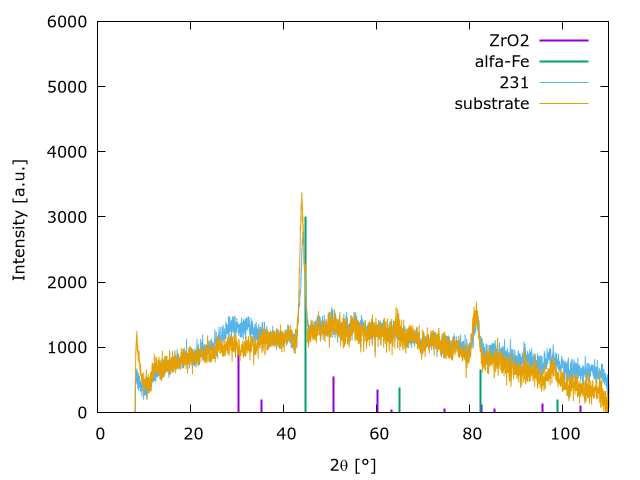
\includegraphics[width=\picwidth]{Pics/xrd.png}
	\caption{XRD spectra}
	\label{fig:xrd}
\end{figure}
\section{Outlook}

Making of the solution for the sol-gel process:
For a single concentrated solution \ml{0.05} of \gls{zrpro} are added while stirring to \ml{4.95} of \gls{buoh} and stirred for \minutes{15}. 
\ml{0.013} (or one molar equvilent of Zr) of \gls{acac} is added to the stirring solution. 
After another \minutes{15} \ml{1} of acetic acid is added and stirred for \minutes{30} to stabilize the solution up to \h{24}. 

The concentration can be increased up to 5 times being stable for a minimum of \h{4}. 
The sol-gel process produces am homogeneous transparent crystalline zirconia oxide layer. 
homogeneity can be mainly controlled via blade velocity and temperature and layers can be stacked.

It should have been alos verglichen with grid search with comparable size
but most time was used to find a vernuenfig base recipe and process

It is still very human 
Der process is - as it the case with all ML and most fitting processes - is very abhaengig von hyper parameters, 
In the current work population size, number of generations, and most importantly boundaries (grenzen). 


%\clearpage
\bibliographystyle{ieeetr}
\bibliography{int}
\end{document}
